\chapter{Experiments and Results}
\label{chap:experiments_and_results}

In this chapter, all the experiments performed using the seed model architecture (\autoref{sec:seed_model}) and NAS with different parameters are described along with their empirical evaluations. The experiments are supported by their qualitative and quantitative results. The validation is run on the validation dataset (TFRecord for validation data) which contains 1,200 AF and 1,200 sinus rhythm files. The results of the selection strategies are discussed and compared.

\subsubsection{Hyperparameters}

Hyperparameters are kept the same throughout the experiments for NAS. For training, \textbf{Adam optimizer} is used with an initial learning rate $4e^{-4}$. A batch size of $32$ is used for training and validation for the seed model as well as for all the models trained during the NAS. The table~\ref{table:hyperparameters} shows the hyperparameters used in the experiments with few changes. The hyperparameter - decay rate is \textbf{not} used for NAS, while all the models for NAS are trained only for $5$ epochs.

\section{Evaluation of Seed models}
\label{sec:seed_model_experiments}

The seed models with the architecture described in Figure~\ref{fig:seed_model_1_n_2} are trained with the hyperparameters defined in table~\ref{table:hyperparameters}. The models are trained for five epochs. The table~\ref{table:seed_model_results} provides the comparison of the results for the two seed models. The results are the average of three runs for both the models. 

\begingroup
\setlength{\tabcolsep}{12pt}
\renewcommand{\arraystretch}{1.5}
\begin{table}[ht]
\normalsize
\resizebox{\textwidth}{!}{%
\centering
\begin{tabular}{|c|c|c|}
\hline
\textbf{Results}     & \textbf{Seed Model 1}  & \textbf{Seed Model 2}  \\ \hline
Number of epochs     & 5                      & 5                      \\ \hline
Number of parameters & 72,777                 & 37,361                 \\ \hline
Training Accuracy    & 0.972                  & 0.943                  \\ \hline
Validation Accuracy  & 0.962                  & 0.946                  \\ \hline
Testing Accuracy     & 0.965                  & 0.949                  \\ \hline
Detection Rate       & 0.990                  & 0.970                  \\ \hline
False Alarm Rate     & 0.060                  & 0.072                  \\ \hline
\end{tabular}}
\caption{Comparison of seed model results}
\label{table:seed_model_results}
\end{table}
\endgroup

As seen from the table, Seed Model 1 produces an average training accuracy of greater than 97\% where as Seed Model 2 produces an average training accuracy of nearly 94.5\%. This result is as per expectations as the decrease in number of parameters would, in general, reduce the accuracy. But in this scenario, the number of parameters is nearly halved between the two models. The validation and the testing accuracy also confirm the training accuracy. This in turn implies that the model is not over-fitted. 

High detection rate and low false alarm rate are also important measures of a good model as they provide us information about the ability of the model to classify new samples. Both the models have resulted in high detection rate (nearly $99 \; \% $ and $97 \; \% $ respectively) and low false alarm rate ($ 6 \; \% $ and $7 \; \% $ respectively). The seed models, thus produce very good results. 

\section{Experiments and results with NAS}
\label{sec:nas_experiments}

Experiments for NAS are run with various configurations in order to evaluate the effect on the results. This includes various selection policies, different number of offspring networks generated per generation, different number of the initial networks, different number of parents for generation and for how many generations should we run the experiment for.

All the experiments were run using the TITAN GPUs provided by the Fraunhofer cluster. Most of the experiments were run on more than one node with multiple GPUs in every node to enable parallel training of the models. Mutation was performed parallelly on several CPUs nodes.

The mutation parameters for the experiments are set as follows:
\begin{itemize}
    \item Threshold accuracy of a parent is set to 80\%. If the accuracy of the parent if less than 80\%, then the mutation rate is high, as the parent is considered to be a bad parent. The child should greatly vary from the parent.
    \item If the accuracy of the parent if greater than 80\% and number of parameters is greater than the average of maximum and minimum parameters, then the mutation rate is moderate as the parent is considered to be a decent parent. This essentially signifies that the offspring architecture should not differ very much from the parent.
    \item If the accuracy of the parent if greater than 80\% and number of parameters is less than the average of maximum and minimum parameters, then the mutation rate is very low as this is considered to be a good parent. This also signifies that the offspring architecture should vary very little from the parent.
\end{itemize}

\subsection{Experiments with Selection strategy - Aging}

For aging, two experiments are run - one with the inclusion of the seed models and another without them. The same setting which is used in Amoebanet, producing one offspring per generation and keeping the population constant is used for these experiments (Table~\ref{table:selection_policy_aging}). We ran few experiments with less than 10 initial networks, but this resulted in reducing the number of parents for selection process. Although, this increased the probability of choosing a good network, it reduced the number of networks to choose from. Hence, we choose the population to be constant at 10 networks. Also, Mutation rate of 70\% - 90\% for a bad parent, 10\% - 30\% for a decent parent and 5\% - 10\% for a good parent is used for these experiments. Accuracy is used as a measure for these experiments.

\begingroup
\setlength{\tabcolsep}{3pt}
\renewcommand{\arraystretch}{1.5}
\begin{table}[ht]
\normalsize
\centering
\begin{tabular}{ccccc}
\hline
\textbf{\begin{tabular}[c]{@{}c@{}}\# epochs\end{tabular}} & \textbf{\begin{tabular}[c]{@{}c@{}}Initial \\ population\end{tabular}} & \textbf{\begin{tabular}[c]{@{}c@{}}\# parents\end{tabular}} & 
\textbf{\begin{tabular}[c]{@{}c@{}}\# offspring\end{tabular}} & 
\textbf{\begin{tabular}[c]{@{}c@{}}\# generations\end{tabular}} \\ \hline \hline
5 & 10 & 5 & 1 & 200 \\
\hline
\end{tabular}
\caption{Parameters for selection strategy - aging}
\label{table:selection_policy_aging}
\end{table}
\endgroup

\begin{figure}[ht!]
    \centering
        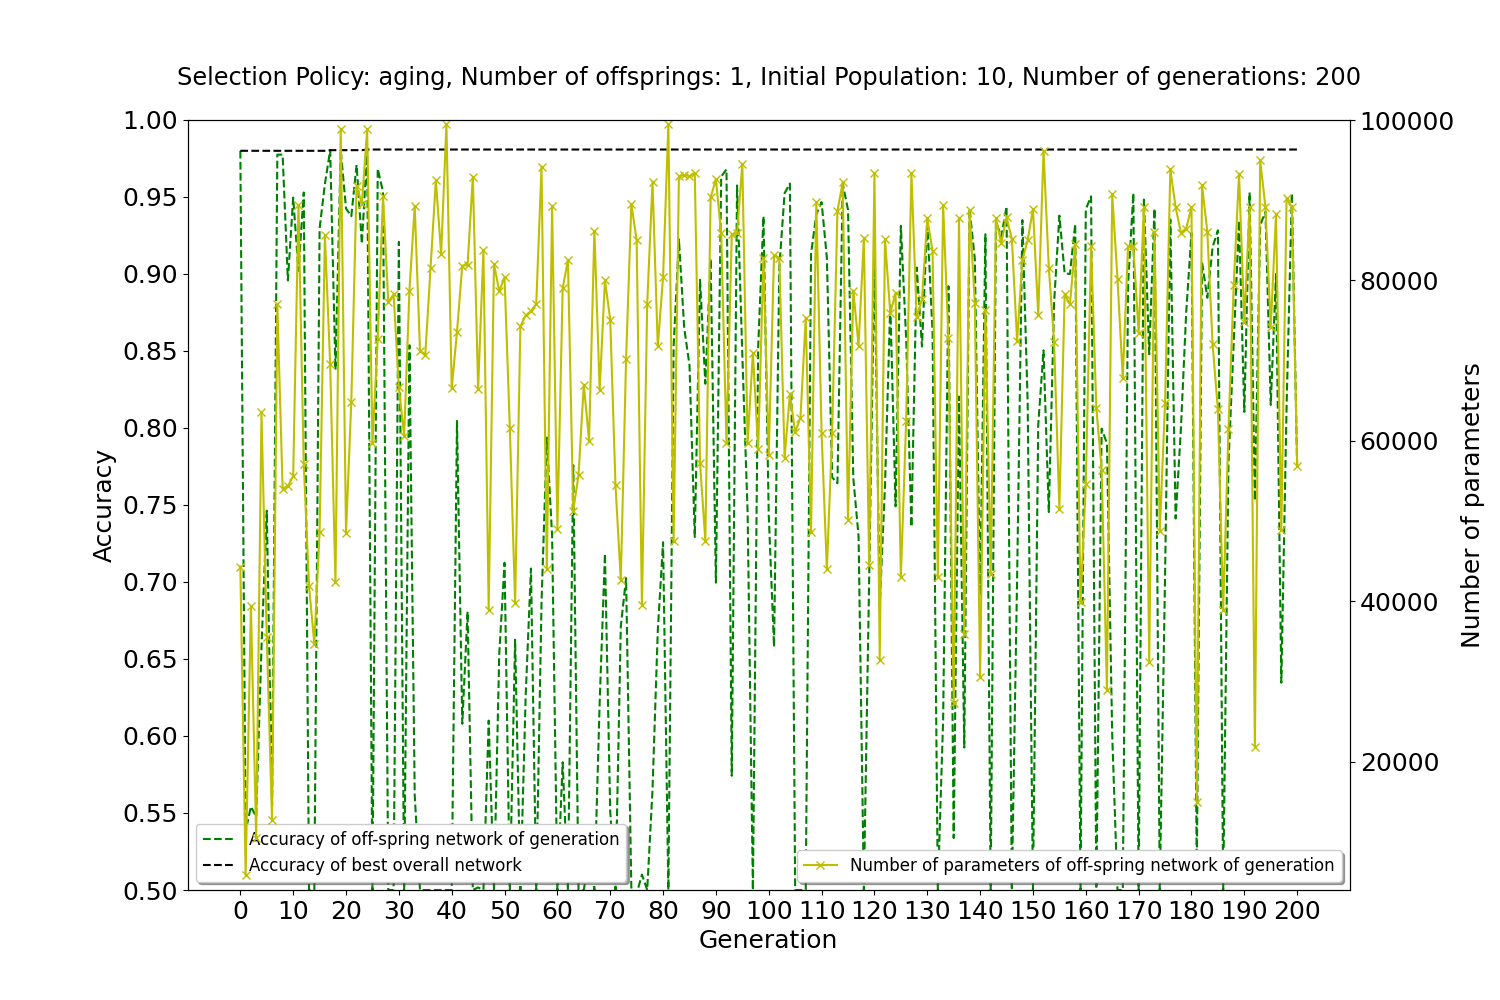
\includegraphics[width=1.0\linewidth, height=8cm]{BachelorMasterThesis/ExperimentsAndResults/Figures/aging/aging_seed_model.png}
        \caption{Aging, with seed models}
        \label{fig:aging_1}
    % \begin{minipage}{1.0\textwidth}
    % \end{minipage}%
\end{figure}
\begin{figure}[ht!]
    \centering
    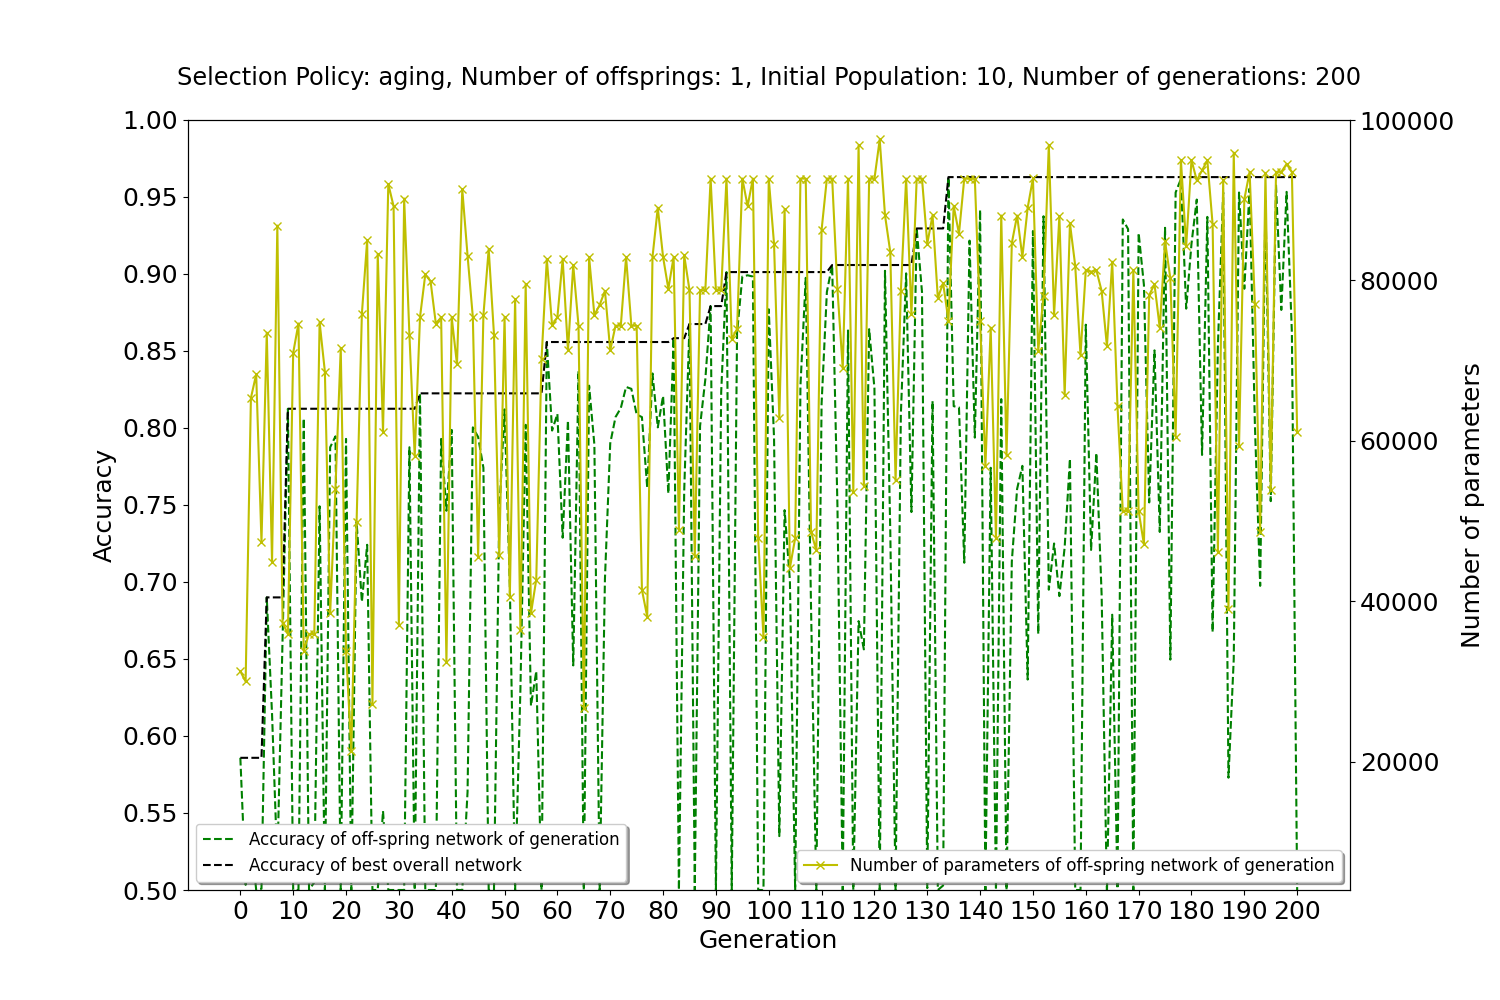
\includegraphics[width=1.0\linewidth, height=8cm]{BachelorMasterThesis/ExperimentsAndResults/Figures/aging/aging_no_seed_model.png}
    \caption{Aging, without seed models}
    \label{fig:aging_2}
    % \begin{minipage}{1.0\textwidth}
    % \end{minipage}
\end{figure}
% \begin{figure}[ht!]
%     \centering
%     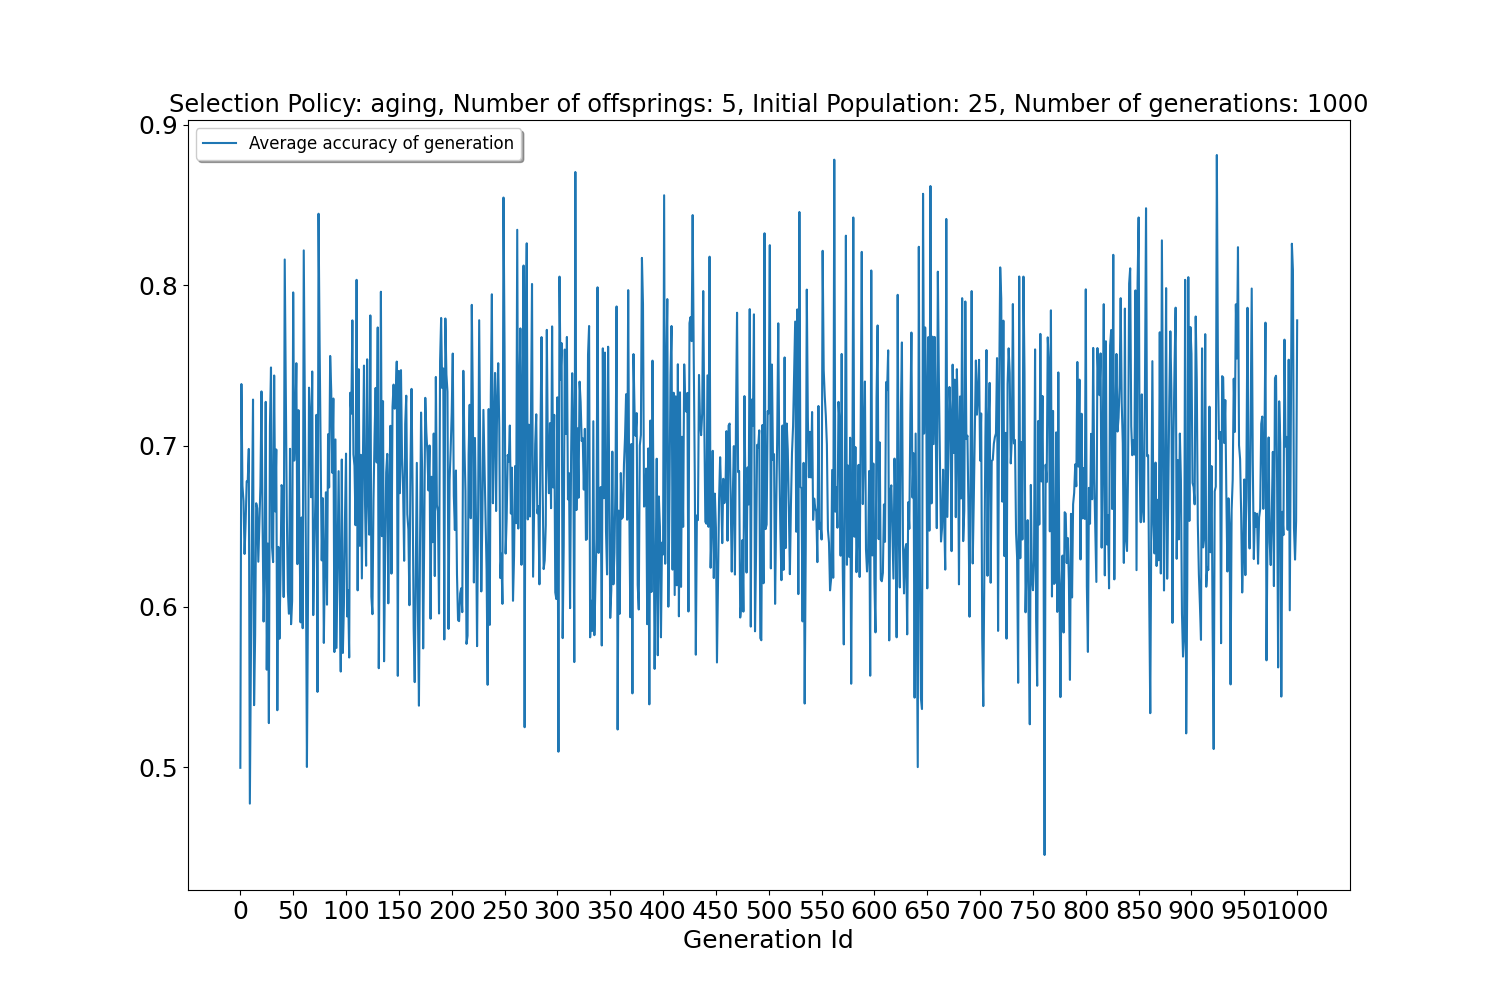
\includegraphics[width=1.0\linewidth, height=4.75cm]{BachelorMasterThesis/ExperimentsAndResults/Figures/generation_1000_aging.png}
%     \caption{Aging - 1000 generations}
%     \label{fig:aging_3}
%     % \begin{minipage}{1.0\textwidth}
%     % \end{minipage} 
% \end{figure}

\subsubsection{Analysis}

For this selection strategy, for the initial population (generation zero), the network with the best accuracy and for the subsequent generations, the accuracy of every offspring generated is used for analysis. Figure~\ref{fig:aging_1} and Figure~\ref{fig:aging_2} show these results. These graphs also show the number of parameters of the networks and the best overall accuracy for these experiments. Figure~\ref{fig:aging_1} clearly explains that our seed model produces very good results and it is very difficult to improve these results. There is a slight increase in accuracy in the 15th generation, but this is at the cost of increase in number of parameters as well. This, in comparison with Figure~\ref{fig:aging_2} where no seed model is used, shows the actual evolving nature of the entire NAS process. This figure explains that the NAS process is always trying to improve the accuracy of the networks, but at the cost of increasing number of parameters. We find a network with very high accuracy between the 130th and 140th generation, but with high number of parameters. This result is expected, as well as other results of these experiments of aging for NAS process, as there is random selection of parents during the selection phase. The results are very noisy with many networks producing 50\% accuracy (networks which don't learn). This is also to be expected from aging during the NAS process, as in these experiments, the process tries to find a network with high accuracy irrespective of the number of parameters. We try to reduce the randomness by using selection policies - all children and selected children.

\subsection{Experiments with Selection strategy - All children, Selected children and Lemonade}

For the selection strategy of all children and selection children, there were many experiments run with the fixed parameters shown in table~\ref{table:selection_policy_all_and_selected_children}. The experiments are run with the accuracy metric as well as the weighted objective metric. We mostly concentrate on using weighted objective metric, as accuracy metric focuses on accuracy and in our scenario, the results should also focus on detection rate, false alarm rate and number of parameters. We choose the initial population to be 10 networks, the same as that in aging. The number of offspring is preset to 20, as this will result in 20 mutated networks every generation and nearly 2000 networks for 100 generations for NAS to explore. The number of parents for selection process for every generation is also preset to 20, the same as the number of offspring.

\begingroup
\setlength{\tabcolsep}{3pt}
\renewcommand{\arraystretch}{1.5}
\begin{table}[b!]
\normalsize
\centering
\begin{tabular}{ccccc}
\hline
\textbf{\begin{tabular}[c]{@{}c@{}}\# \\ epochs\end{tabular}} & \textbf{\begin{tabular}[c]{@{}c@{}}Initial \\ population\end{tabular}} & \textbf{\begin{tabular}[c]{@{}c@{}}\# \\ parents\end{tabular}} & \textbf{\begin{tabular}[c]{@{}c@{}}\# \\ offspring\end{tabular}} & \textbf{\begin{tabular}[c]{@{}c@{}}\# \\ generations\end{tabular}} \\ \hline \hline
5 & 10 & 20 & 20 & 100 \\  
\hline
\end{tabular}
\caption{Parameters for selection strategy - All children, Selected children}
\label{table:selection_policy_all_and_selected_children}
\end{table}
\endgroup

The experiments are run with variations in mutation rates (MR) and different weights assigned to the metrics while using weighted objectives. These experiments help us to observe the effect of changes in the weights as well as mutation rate in the performance of the NAS process. We try to concentrate on reducing the number of parameters keeping in mind that the objective is to have models with least number of parameters with detection rate greater than 90\% and false alarm rate less than 20\% simultaneously. This would also result in good accuracy, as high detection rate and low false alarm rate are analogous to good accuracy. The mutation rate and weights for every experiment are mentioned along with the results.

For all children, we run an experiment with the lower and upper bound for mutation rate, for a bad parent, set to 70\% and 90\% respectively, as this would facilitate the offspring to greatly vary from the parent. For a decent parent, the upper and lower bound is 10\% and 30\% where as for a good parent it is 5\% and 10\%, as this would make the offspring not to vary a lot from the parent (Table~\ref{table:all_children_3_3_1_mutation_rate_10_30_5_10}). After running an experiment with the weights for the metrics - detection rate, false alarm rate and number of parameters set to equal weights of one, which did not produce great results, we set these metrics values to three, three and one respectively. 

Increasing the weights for detection rate and false alarm rate would penalize those networks with detection rate below and false alarm rate above the threshold values respectively. This would also emphasize more on the detection rate and false alarm rate for the best weighted network (BWN), while trying to reduce the number of parameters. The results for these experiments with and without the seed model are mentioned in Figure~\ref{fig:all_children_3_3_1_seed_model_mutation_rate_10_30_5_10} and Figure~\ref{fig:all_children_3_3_1_no_seed_model_mutation_rate_10_30_5_10}, respectively. The x-axis for both the graphs define the generation number where as, the y-axis define the detection rate/false alarm rate on one axis and number of parameters on the other. 

\begingroup
\setlength{\tabcolsep}{5pt}
\renewcommand{\arraystretch}{1.2}
\begin{table}[h!]
\normalsize
\resizebox{\textwidth}{!}{%
\centering
\begin{tabular}{cccccc}
\hline
\begin{tabular}[c]{@{}c@{}}MR for\\ bad\\ parent\end{tabular} & 
\begin{tabular}[c]{@{}c@{}}MR for \\ decent\\ parent\end{tabular} & 
\begin{tabular}[c]{@{}c@{}}MR for \\ good\\ parent\end{tabular} & 
\begin{tabular}[c]{@{}c@{}}Weight \\ for \\ detection\\  rate\end{tabular} & \begin{tabular}[c]{@{}c@{}}Weight \\ for \\ false alarm \\ rate\end{tabular} & \begin{tabular}[c]{@{}c@{}}Weight \\ for \\ number of \\ parameters\end{tabular} \\ \hline \hline
70\% - 90\% & 10\% - 30\% & 5\% - 10\% & 3 & 3 & 1 \\ 
\hline
\end{tabular}}
\caption{Mutation rate (MR) and weights for metrics}
\label{table:all_children_3_3_1_mutation_rate_10_30_5_10}
\end{table}
\endgroup

\begin{figure}[ht!]
    \centering
        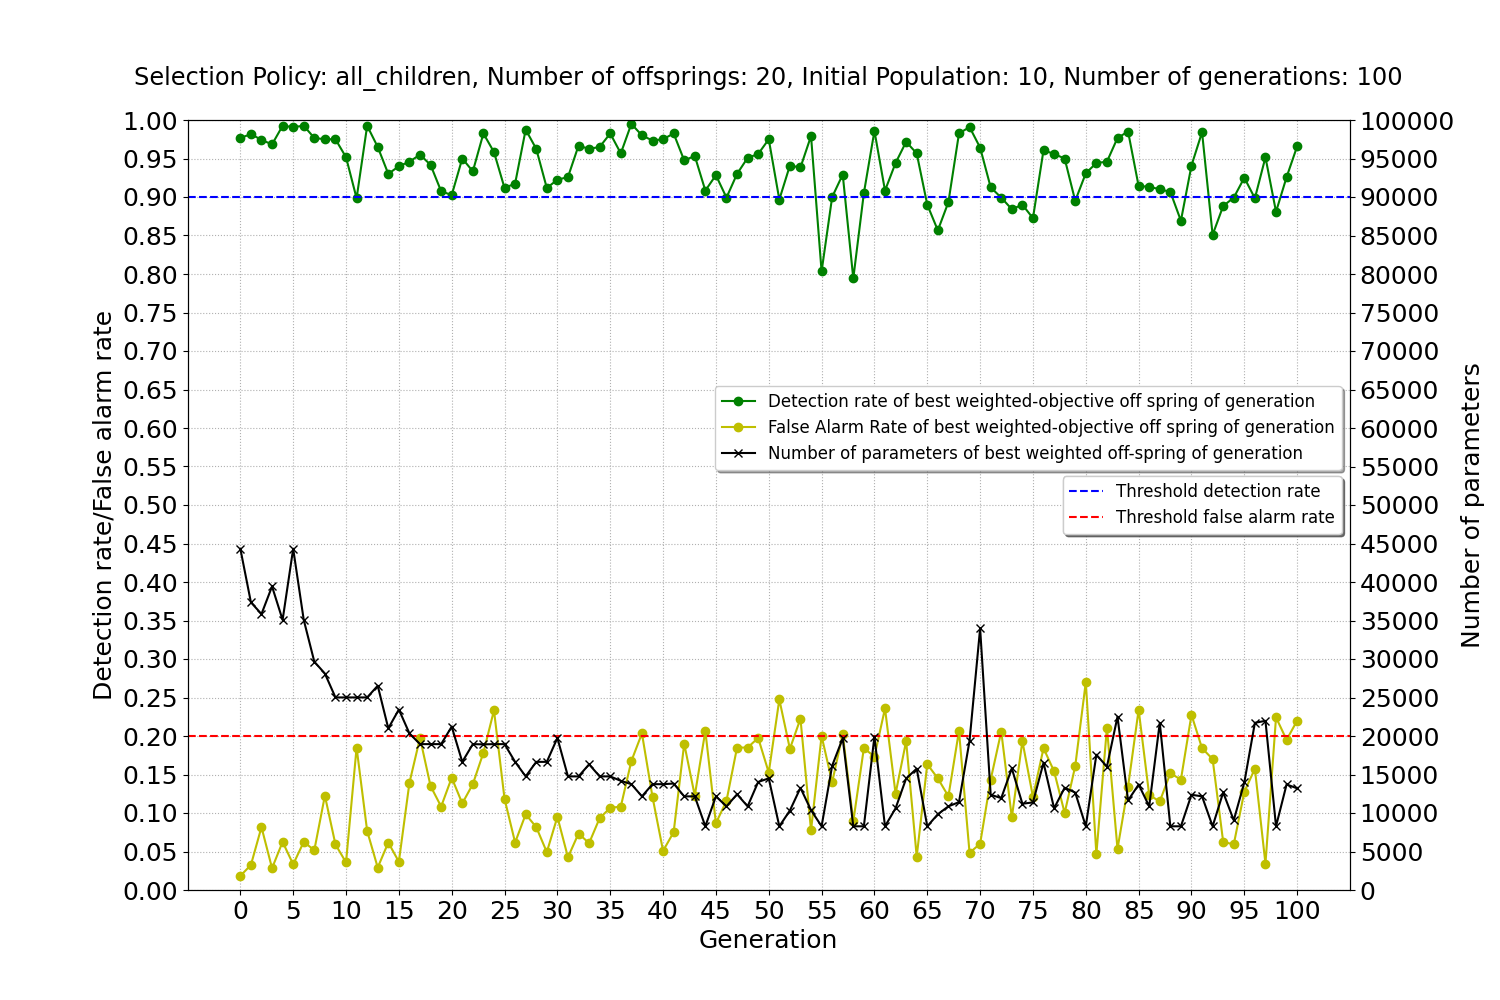
\includegraphics[width=1.0\linewidth, height=7cm]{BachelorMasterThesis/ExperimentsAndResults/Figures/all_children/all_children_3_3_1_seed_model_mutation_rate_10_30_5_10.png}
        \caption{NAS with selection strategy - all children with seed model}
        \label{fig:all_children_3_3_1_seed_model_mutation_rate_10_30_5_10}
    % \begin{minipage}{1.0\textwidth}
    % \end{minipage}%
\end{figure}

\begin{figure}[ht!]
    \centering
        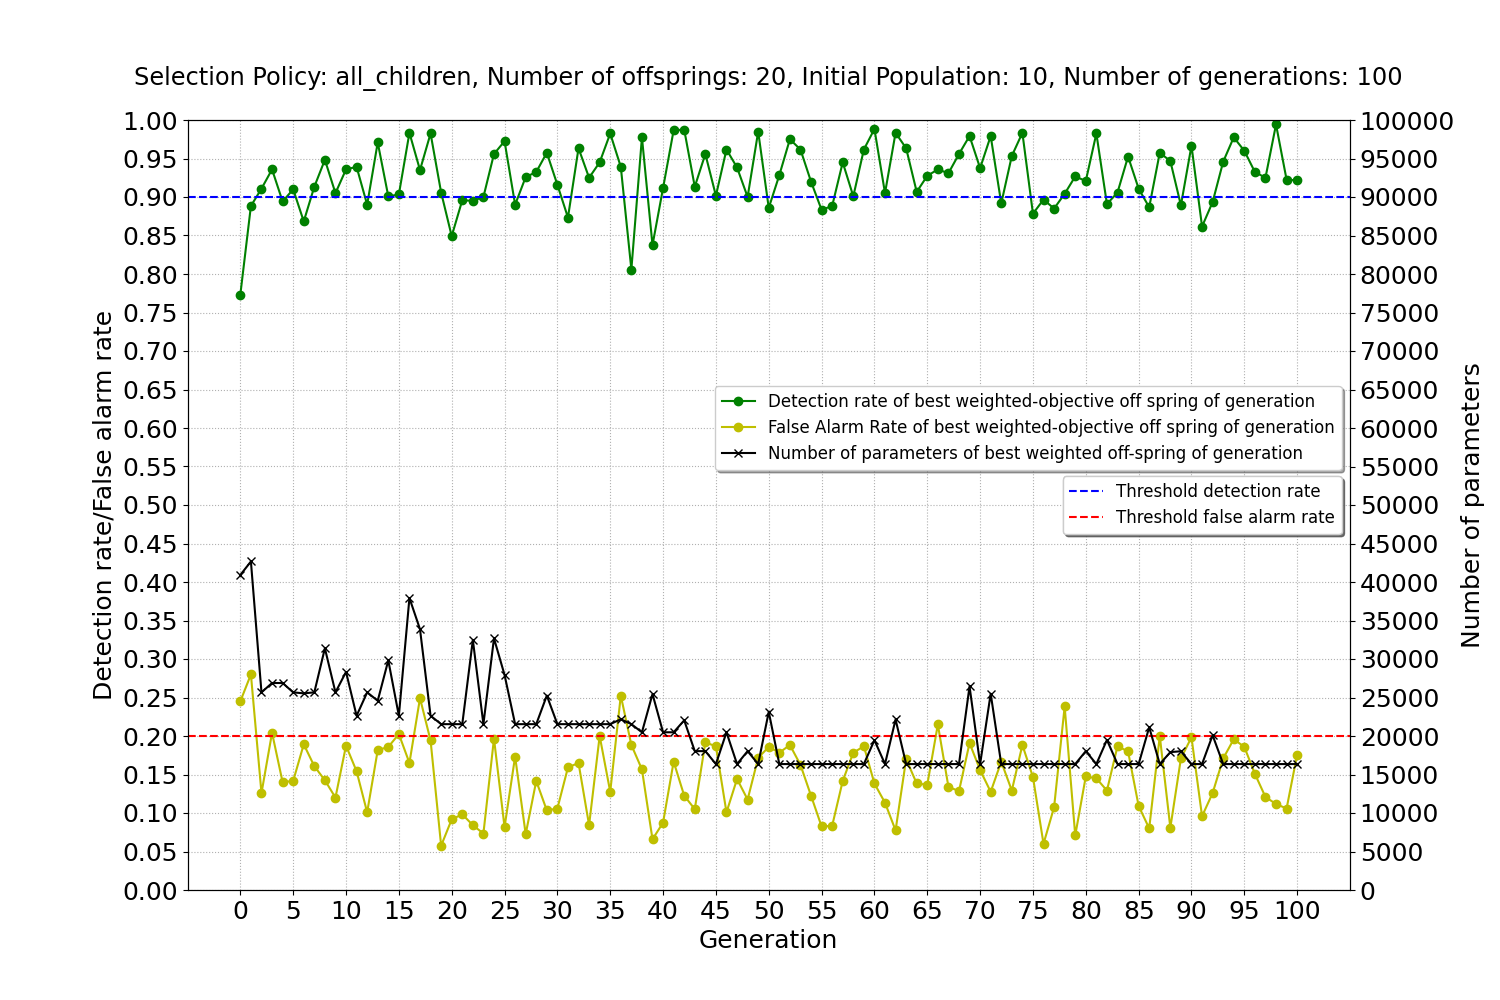
\includegraphics[width=1.0\linewidth, height=7cm]{BachelorMasterThesis/ExperimentsAndResults/Figures/all_children/all_children_3_3_1_no_seed_model_mutation_rate_10_30_5_10.png}
        \caption{NAS with selection strategy - all children without seed model}
        \label{fig:all_children_3_3_1_no_seed_model_mutation_rate_10_30_5_10}
    % \begin{minipage}{1.0\textwidth}
    % \end{minipage}%
\end{figure}

Although the seed model (generation 0) has very high detection rate and low false alarm rate, it still has more than 40,000 parameters. The evolution process, using these weights, tries to further reduce the number of parameters but by keeping detection rate and false alarm rate above and below the threshold values. For the BWN of every generation, the number of parameters reach below 20,000 mark in the 17th generation and remain below this value for most of following generations. Further, there are nearly 15\% BWNs that have less than 10,000 parameters for this experiment with the network in the generation 59 having around 8,000 parameters with other metrics above and below the threshold. There are exceptions for few generations, but the general downward trend of the number of parameters is evident from Figure~\ref{fig:all_children_3_3_1_seed_model_mutation_rate_10_30_5_10}.

When no seed model is used, the evolution process starts with random models with BWN producing nearly 75\% detection rate and 25\% false alarm rate for the initial population (generation 0). This improves in the later generations as the detection rate and false alarm rate reach above and below the threshold values in the third generation, although it takes another eight generations (in the 11th generation) to reduce the number of parameters further. The number of parameters reach below 20,000 mark in the 43th generation (26 more generations than in the experiment with seed model) and reaches the minimum of nearly 16,000 in the 45th generation maintaining the detection rate and false alarm rate above and below the threshold values. For the majority of the next generations, the number of parameters for the BWN remains the same at around 16,000 (as shown in Figure~\ref{fig:all_children_3_3_1_no_seed_model_mutation_rate_10_30_5_10}).

We can observe that the experiment with the seed model produces BWN models with lower number of parameters (15\% BWN models have less than 10,000 parameters) when compared to that without the seed model. The detection rate and false alarm rate for both the experiments follow almost the same pattern of trying to maintain values above and below the threshold values. The evolution process for the two experiments produces nearly 75\% and 50\% BWNs with high detection rate and low false alarm rate with less than 20,000 parameters, less than half of the number of parameters of the seed model.

To observe the effect of variations in mutation rate, we run an experiment (without the seed model) with changes in mutation rate but with the same weights used in the previous experiments. The lower bound for mutation rate for a decent parent is increased by 5\%, whereas both the lower and upper bound for the good parent is increased by 5\% (described in table~\ref{table:all_children_3_3_1_mutation_rate_15_30_10_15}). This would increase the variations for a child from a decent and a good parent. The result is displayed in Figure~\ref{fig:all_children_3_3_1_no_seed_model_mutation_rate_15_30_10_15}.


\begingroup
\setlength{\tabcolsep}{5pt}
\renewcommand{\arraystretch}{1.2}
\begin{table}[!ht]
\normalsize
\resizebox{\textwidth}{!}{%
\centering
\begin{tabular}{cccccc}
\hline
\begin{tabular}[c]{@{}c@{}}MR for\\ bad\\ parent\end{tabular} & \begin{tabular}[c]{@{}c@{}}MR for \\ decent\\ parent\end{tabular} & \begin{tabular}[c]{@{}c@{}}MR for \\ good\\ parent\end{tabular} & \begin{tabular}[c]{@{}c@{}}Weight \\ for \\ detection\\  rate\end{tabular} & \begin{tabular}[c]{@{}c@{}}Weight \\ for \\ false alarm \\ rate\end{tabular} & \begin{tabular}[c]{@{}c@{}}Weight \\ for \\ number of \\ parameters\end{tabular} \\ \hline \hline
70\% - 90\% & 15\% - 30\% & 10\% - 15\% & 3 & 3 & 1 \\ 
\hline
\end{tabular}}
\caption{Mutation rate and weights for metrics}
\label{table:all_children_3_3_1_mutation_rate_15_30_10_15}
\end{table}
\endgroup

\begin{figure}[h!]
    \centering
        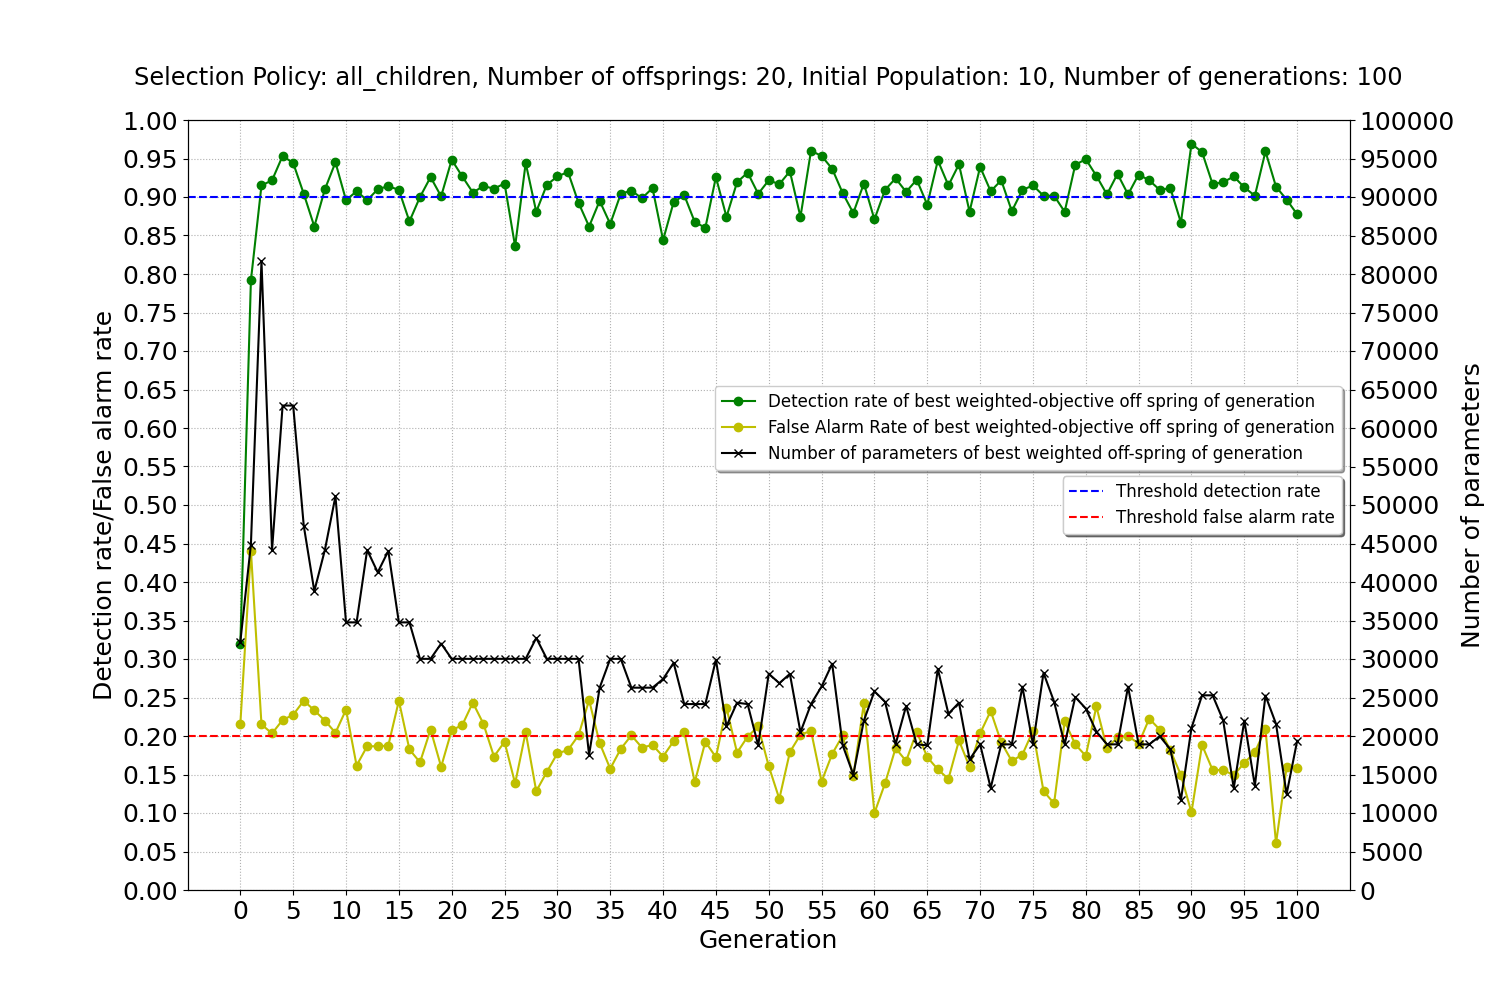
\includegraphics[width=1.0\linewidth, height=7cm]{BachelorMasterThesis/ExperimentsAndResults/Figures/all_children/all_children_3_3_1_no_seed_model_mutation_rate_15_30_10_15.png}
        \caption{NAS with selection strategy - all children without seed model with higher mutation rate}
        \label{fig:all_children_3_3_1_no_seed_model_mutation_rate_15_30_10_15}
    % \begin{minipage}{1.0\textwidth}
    % \end{minipage}%
\end{figure}

In this experiment, the detection rate and the false alarm rate goes above and below the threshold values in the 11th generation (when compared to 3rd generation in the previous experiment). Also, the number of parameters for this network is nearly 35,000 which is higher when compared to the previous experiment. The number of parameters for the BWN does not remain constant, which was the case in the previous experiment. Also, the number of parameters does not decrease at the same rate. It can also be observed that nearly 60\% of the detection rate and false alarm rates are above and below the threshold values for the BWN where as, in the previous experiments, nearly 75\% of the detection rate and false alarm rate values were, respectively, above and below the threshold values. This experiment, thus, tell us that choosing the lower mutation rate is essential for producing good networks. 

Modification in weights also impacts the performance of the evolution process. To observe these effects, two more experiments, one with seed models and another without it is run with the weights described in table ~\ref{table:all_children_5_5_1_mutation_rate_10_30_5_10}. The weight for detection rate and false alarm rate is increased to 5 (from 3), as this would penalize those networks with lower than threshold detection rate and higher than threshold false alarm rate, more, when compared to previous experiment. With these changes, the expectation is to find the BWNs to have better detection rate and lower false alarm rate with less number of parameters and also to find more such networks when compared to the previous experiments  (Figure~\ref{fig:all_children_3_3_1_seed_model_mutation_rate_10_30_5_10} and Figure~\ref{fig:all_children_3_3_1_no_seed_model_mutation_rate_10_30_5_10}). The results for these experiments are displayed in Figure~\ref{fig:all_children_5_5_1_seed_model_mutation_rate_10_30_5_10} and Figure~\ref{fig:all_children_5_5_1_no_seed_model_mutation_rate_10_30_5_10}.

\begingroup
\setlength{\tabcolsep}{5pt}
\renewcommand{\arraystretch}{1.2}
\begin{table}[h!]
\normalsize
\resizebox{\textwidth}{!}{%
\centering
\begin{tabular}{cccccc}
\hline
\begin{tabular}[c]{@{}c@{}}MR for\\ bad\\ parent\end{tabular} & \begin{tabular}[c]{@{}c@{}}MR for \\ decent\\ parent\end{tabular} & \begin{tabular}[c]{@{}c@{}}MR for \\ good\\ parent\end{tabular} & \begin{tabular}[c]{@{}c@{}}Weight \\ for \\ detection\\  rate\end{tabular} & \begin{tabular}[c]{@{}c@{}}Weight \\ for \\ false alarm \\ rate\end{tabular} & \begin{tabular}[c]{@{}c@{}}Weight \\ for \\ number of \\ parameters\end{tabular} \\ \hline \hline
70\% - 90\% & 10\% - 30\% & 5\% - 10\% & 5 & 5 & 1 \\ 
\hline
\end{tabular}}
\caption{Mutation rate and weights for metrics}
\label{table:all_children_5_5_1_mutation_rate_10_30_5_10}
\end{table}
\endgroup

The results also validate this intuition as increasing the weights for detection rate and false alarm rate increase the detection rate and decrease the false alarm rate for the BWNs. Nearly 90\% of the networks for the seed model and 80\% without seed model have detection rate and false rate above and below the threshold values. For the seed model experiment, the number of parameters reduce to below 20,000 mark in the 16th generation (compared with around the 20th generation in the previous experiment), where as for the experiment without seed model, this result is achieved after the 60th generation (compared to 43rd in the previous experiment). For both these networks, the detection rate is higher and false alarm rate is lower when compared to the previous experiment. Also, 35\% of the networks for the experiment with the seed model have less than 10,000 parameters (compared to 15\% in the previous experiment). There are 8\% networks with nearly 10,000 parameters for the experiment without the seed model, which was not the case in the previous experiment (in which the network with least number of parameters has nearly 16,000 parameters). Further increasing the weights did not provide good results as the number of parameters for the BWN also increased. 

\begin{figure}[ht!]
    \centering
        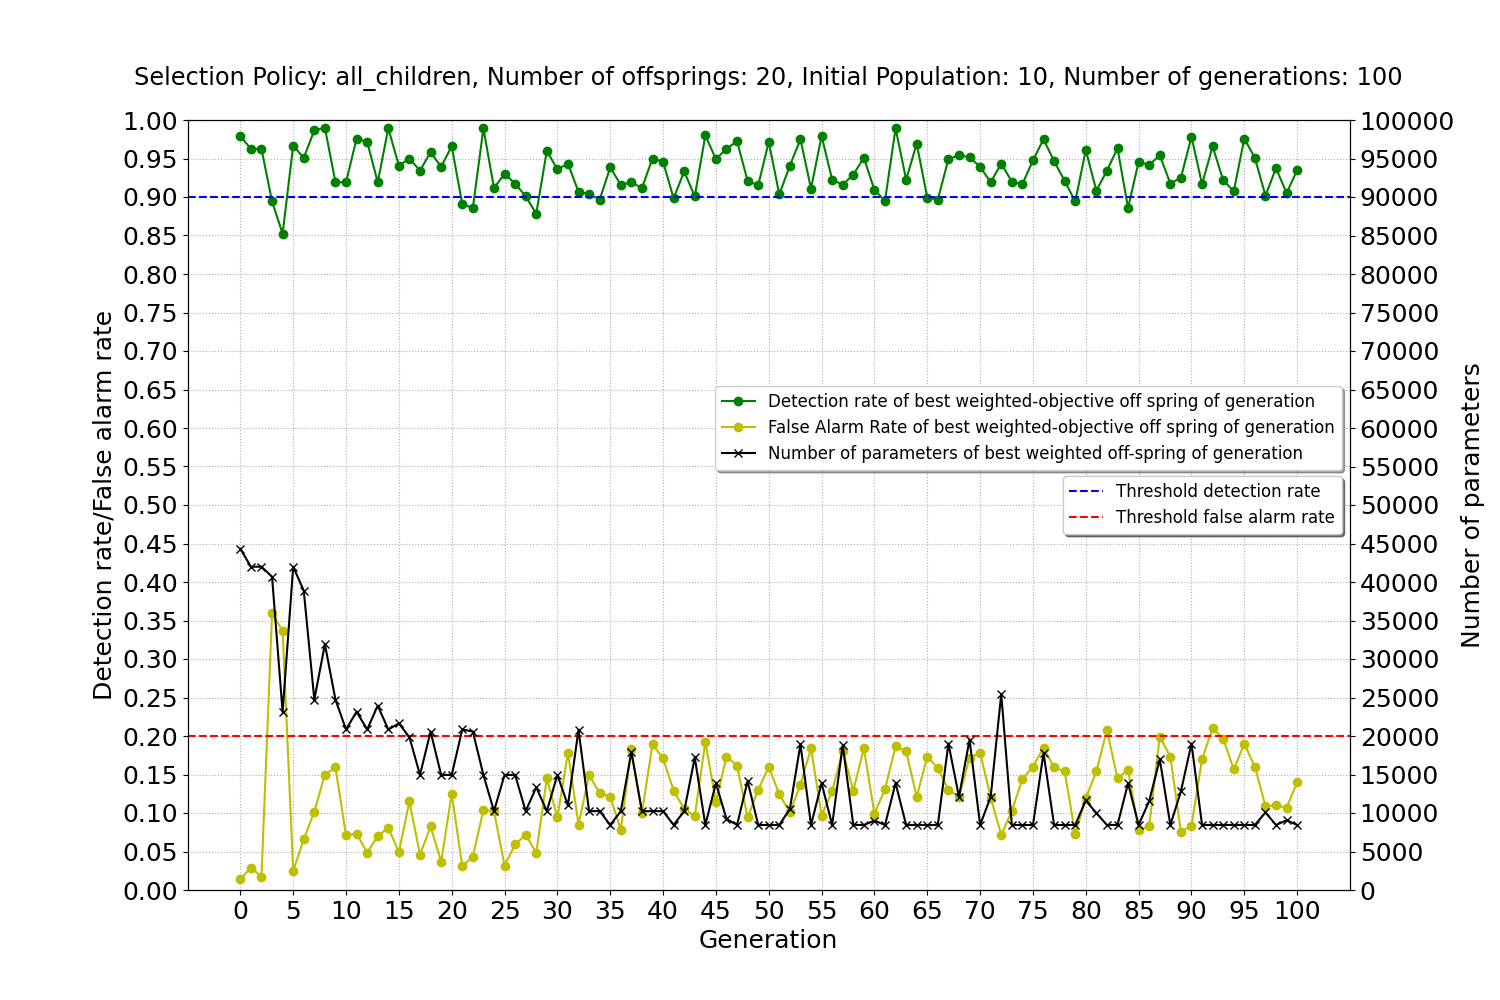
\includegraphics[width=1.0\linewidth, height=7.5cm]{BachelorMasterThesis/ExperimentsAndResults/Figures/all_children/all_children_5_5_1_seed_model_mutation_rate_10_30_5_10.png}
        \caption{NAS with selection strategy - all children with seed model with higher weights for detection rate and false alarm rate}
        \label{fig:all_children_5_5_1_seed_model_mutation_rate_10_30_5_10}
    % \begin{minipage}{1.0\textwidth}
    % \end{minipage}%
\end{figure}

\begin{figure}[h!]
    \centering
        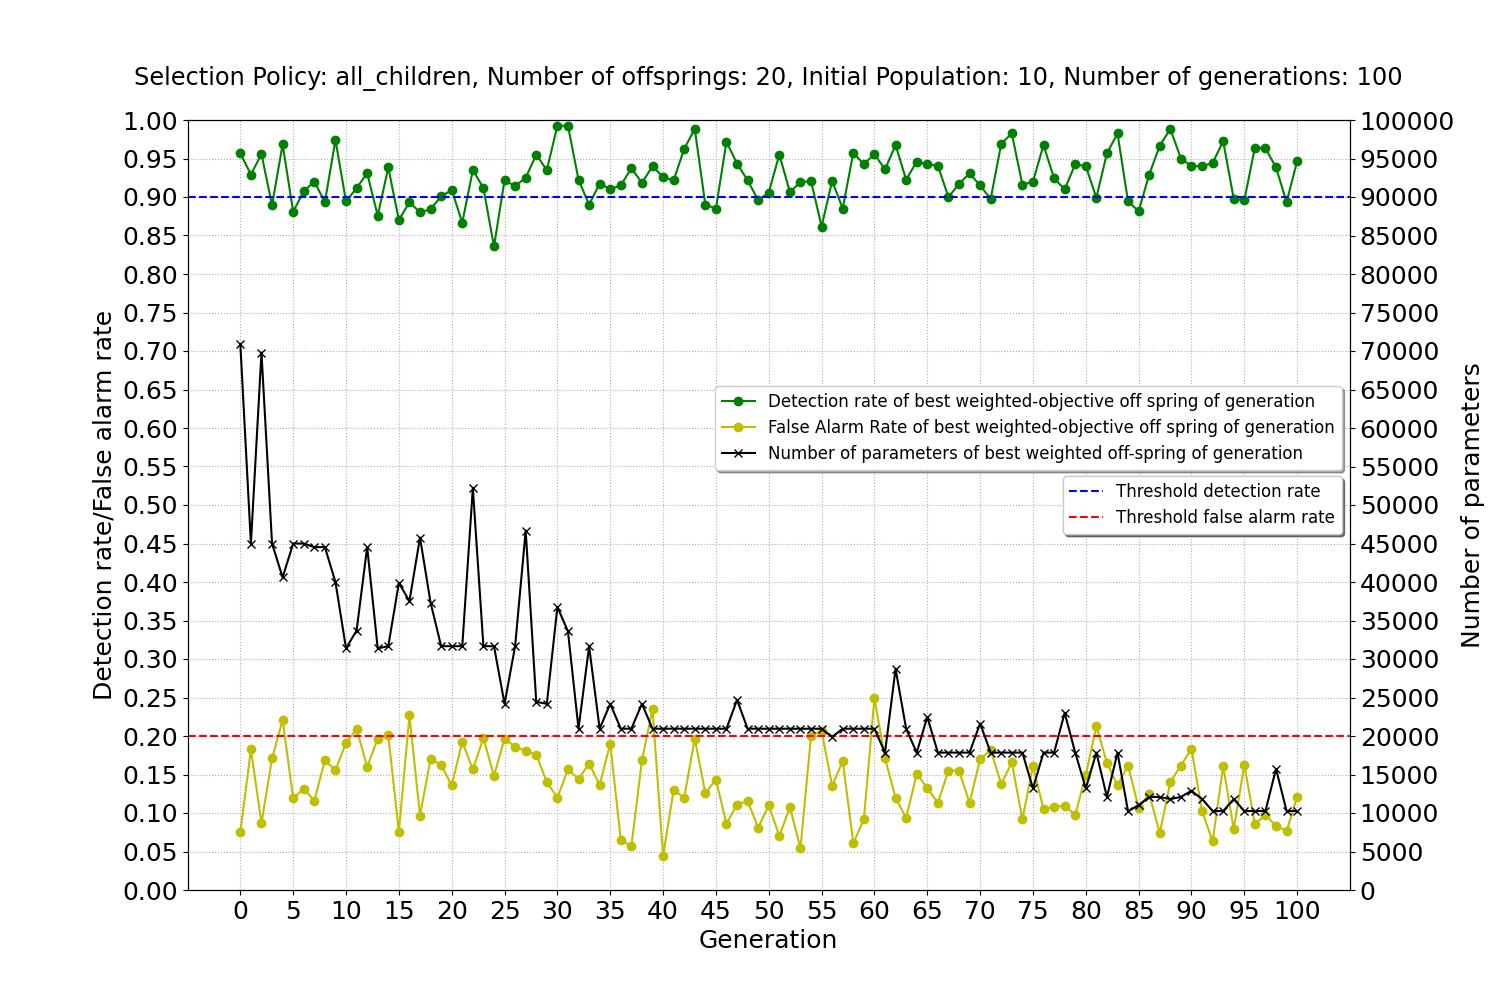
\includegraphics[width=1.0\linewidth, height=7.5cm]{BachelorMasterThesis/ExperimentsAndResults/Figures/all_children/all_children_5_5_1_no_seed_model_mutation_rate_10_30_5_10.png}
        \caption{NAS with selection strategy - all children without seed model with higher weights for detection rate and false alarm rate}
        \label{fig:all_children_5_5_1_no_seed_model_mutation_rate_10_30_5_10}
    % \begin{minipage}{1.0\textwidth}
    % \end{minipage}%
\end{figure}

To further see the effects of weights for the evolution process, one more experiment where we reduce the weight for detection rate and false alarm rate to 3 (from 5) and increase the weight for the number of parameters to 5 (from 1) (Table~\ref{table:all_children_3_3_5_mutation_rate_10_30_5_10}) is run. In this experiment, more bias is provided to number of parameters when compared to detection rate and false alarm rate, which means that the networks with more parameters will be penalised higher than the other metrics. This would also result in the BWN to have more importance to number of parameters and less to detection rate and false alarm rate. The results are provided in Figure~\ref{fig:all_children_3_3_5_no_seed_model_mutation_rate_10_30_5_10}. The results are not very good as during the selection phase, the algorithm gives more emphases to parents with less number of parameters even if they don't have high detection rate and low false alarm rate, thus reducing the probability of producing a good offspring network. This experiment also informs that more significance should be given to detection rate and false alarm rate than the number of parameters. 

\begingroup
\setlength{\tabcolsep}{5pt}
\renewcommand{\arraystretch}{1.2}
\begin{table}[h!]
\normalsize
\resizebox{\textwidth}{!}{%
\centering
\begin{tabular}{cccccc}
\hline
\begin{tabular}[c]{@{}c@{}}MR for\\ bad\\ parent\end{tabular} & \begin{tabular}[c]{@{}c@{}}MR for \\ decent\\ parent\end{tabular} & \begin{tabular}[c]{@{}c@{}}MR for \\ good\\ parent\end{tabular} & \begin{tabular}[c]{@{}c@{}}Weight \\ for \\ detection\\  rate\end{tabular} & \begin{tabular}[c]{@{}c@{}}Weight \\ for \\ false alarm \\ rate\end{tabular} & \begin{tabular}[c]{@{}c@{}}Weight \\ for \\ number of \\ parameters\end{tabular} \\ \hline \hline
70\% - 90\% & 10\% - 30\% & 5\% - 10\% & 3 & 3 & 5 \\ 
\hline
\end{tabular}}
\caption{Mutation rate (MR) and weights for metrics}
\label{table:all_children_3_3_5_mutation_rate_10_30_5_10}
\end{table}
\endgroup

\begin{figure}[ht!]
    \centering
        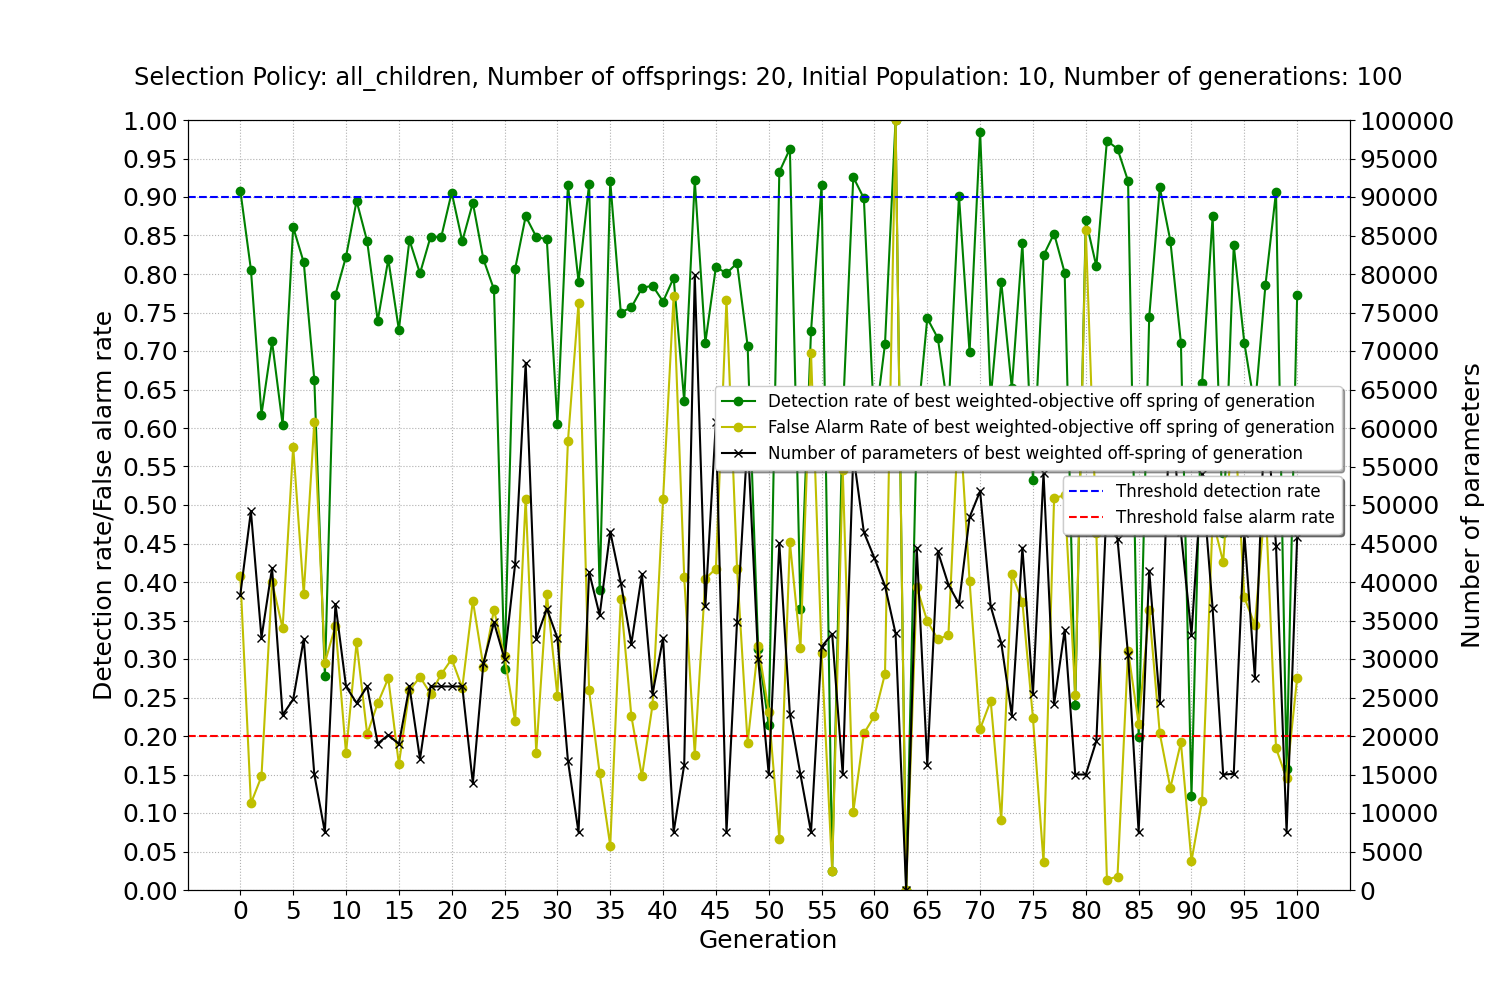
\includegraphics[width=1.0\linewidth, height=7.5cm]{BachelorMasterThesis/ExperimentsAndResults/Figures/all_children/all_children_3_3_5_no_seed_model_mutation_rate_10_30_5_10.png}
        \caption{NAS with selection strategy - all children without seed model}
        \label{fig:all_children_3_3_5_no_seed_model_mutation_rate_10_30_5_10}
    % \begin{minipage}{1.0\textwidth}
    % \end{minipage}%
\end{figure}

We run an experiment for selection strategy - lemonade. The threshold accuracy for mutation rate for a good parent is set at 80\%, the same as previous experiments. The lower and upper bound for mutation rate for a bad parent to 70\% and 90\% respectively, the same as previous experiment. This would facilitate the offspring to greatly vary from the parent. For a decent parent, the upper and lower bound is 10\% and 30\% where as for a good parent it is 5\% and 10\%, again the same as the previous experiments. These parameters are shown in table \ref{table:pareto_front}. We run this experiment with the accuracy measure as the Pareto front is performed on number of parameters and validation error (1 - accuracy) \cite{elsken2018efficient}. The result is shown in Figure~\ref{fig:pareto_front}. The Pareto front is plotted for generations 1, 10, 50 and 100, as this would indicate, roughly, the progress of the evolution process. 

As expected from the algorithm, networks along the Pareto-front are added continuously over the generations. We can also observe that the number of parameters and validation error gradually decrease for networks on the Pareto front line, thus shifting the line lower with the increase in the number of generations. This is also according to the intuition that lemonade tries to balance the number of parameters with that of the validation error. In generation 100, we have many networks with parameters between 25,000 and 30,000 with validation error between 5\% and 10\%. After obtaining this graph, it is up to the user to select a network according to his choice of choosing a network with less number of parameters or one with less validation error.

\begingroup
\setlength{\tabcolsep}{5pt}
\renewcommand{\arraystretch}{1.5}
\begin{table}[ht!]
\normalsize
\centering
\begin{tabular}{ccc}
\hline
\begin{tabular}[c]{@{}c@{}}MR for\\ bad parent\end{tabular} &
\begin{tabular}[c]{@{}c@{}}MR for\\ decent parent\end{tabular} &
\begin{tabular}[c]{@{}c@{}}MR for\\ good parent\end{tabular} \\ \hline \hline
 70\% - 90\% & 10\% - 30\% & 5\% - 10\% \\ \hline
\end{tabular}
\caption{Mutation rate (MR) for lemonade, with accuracy as measure}
\label{table:pareto_front}
\end{table}
\endgroup

\begin{figure}[ht!]
    \centering
        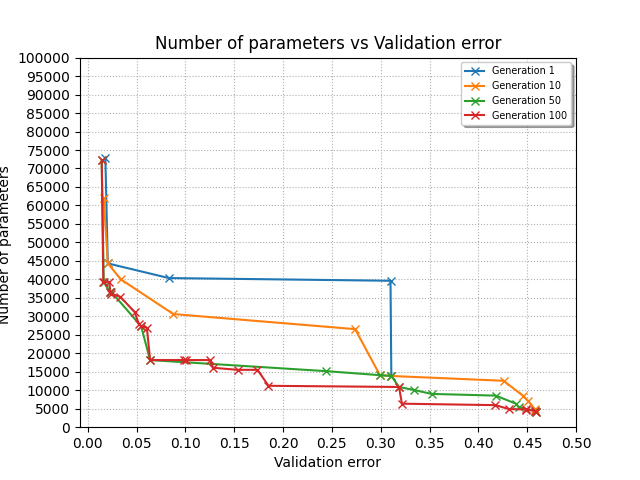
\includegraphics[width=1.0\linewidth, height=7.5cm]{BachelorMasterThesis/ExperimentsAndResults/Figures/lemonade/pareto_front_accuracy.png}
        \caption{NAS with selection strategy - lemonade with seed model, with accuracy as measure}
        \label{fig:pareto_front}
    % \begin{minipage}{1.0\textwidth}
    % \end{minipage}%
\end{figure}

Figures~\ref{fig:aging_networks_least_nop}, ~\ref{fig:selected_children_networks_least_nop}, ~\ref{fig:all_children_networks_least_nop}, ~\ref{fig:all_children_networks_least_nop_all_less_than_10000} show the networks for various selection policies with least number of parameters for detection rate greater than 90\% and false alarm rate less than 20\%. These results are obtained from the various experiments run with various mutation rate and weights. 

From these graphs, we can see that aging does not greatly improve the results from that of the seed models as the network with least number of parameters has around 30,000 parameters but also with less detection rate and higher false alarm rate Figures~\ref{fig:aging_networks_least_nop}.

\begin{figure}[ht!]
    \centering
        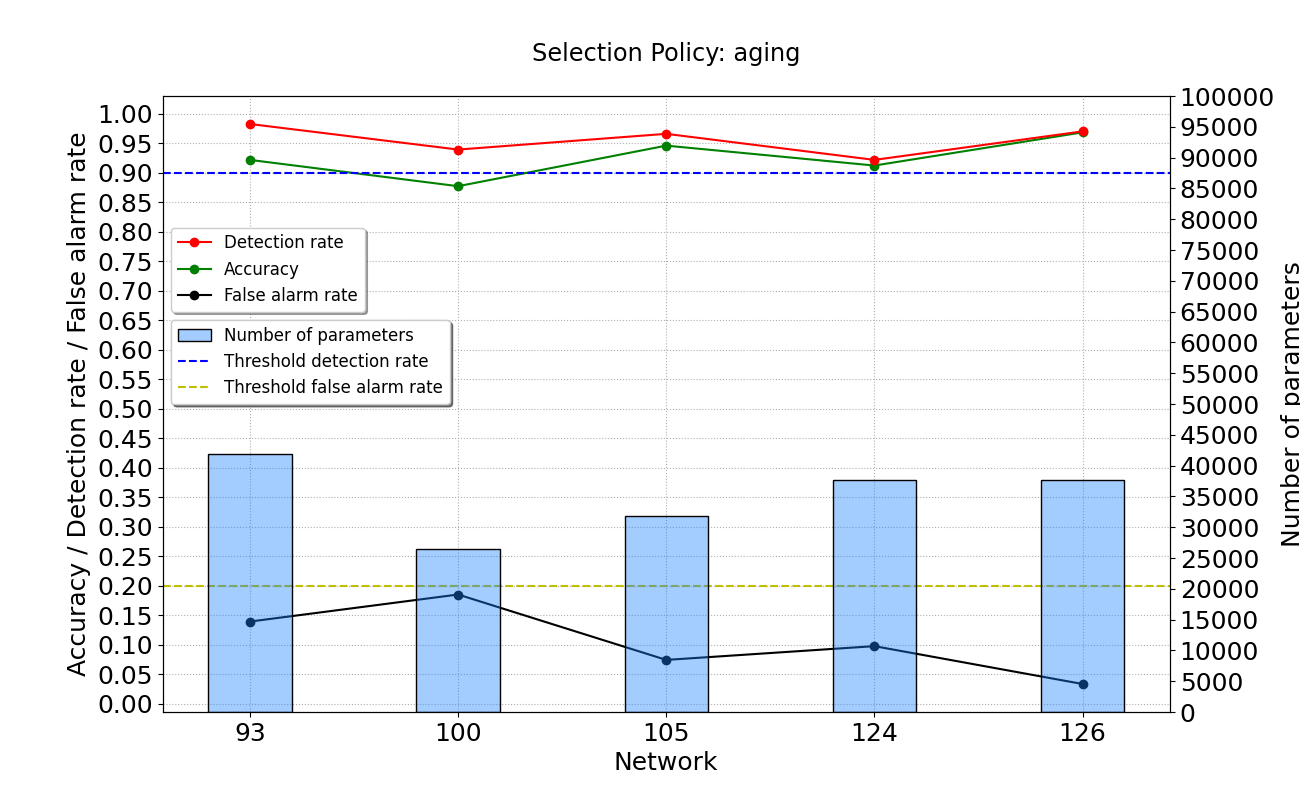
\includegraphics[width=1.0\linewidth, height=8cm]{BachelorMasterThesis/ExperimentsAndResults/Figures/aging/aging_networks_least_nop.png}
        \caption{Aging - network with least parameters for detection rate greater than 90\% and false alarm rate less than 20\%}
        \label{fig:aging_networks_least_nop}
    % \begin{minipage}{1.0\textwidth}
    % \end{minipage}%
\end{figure}

\begin{figure}[ht!]
    \centering
        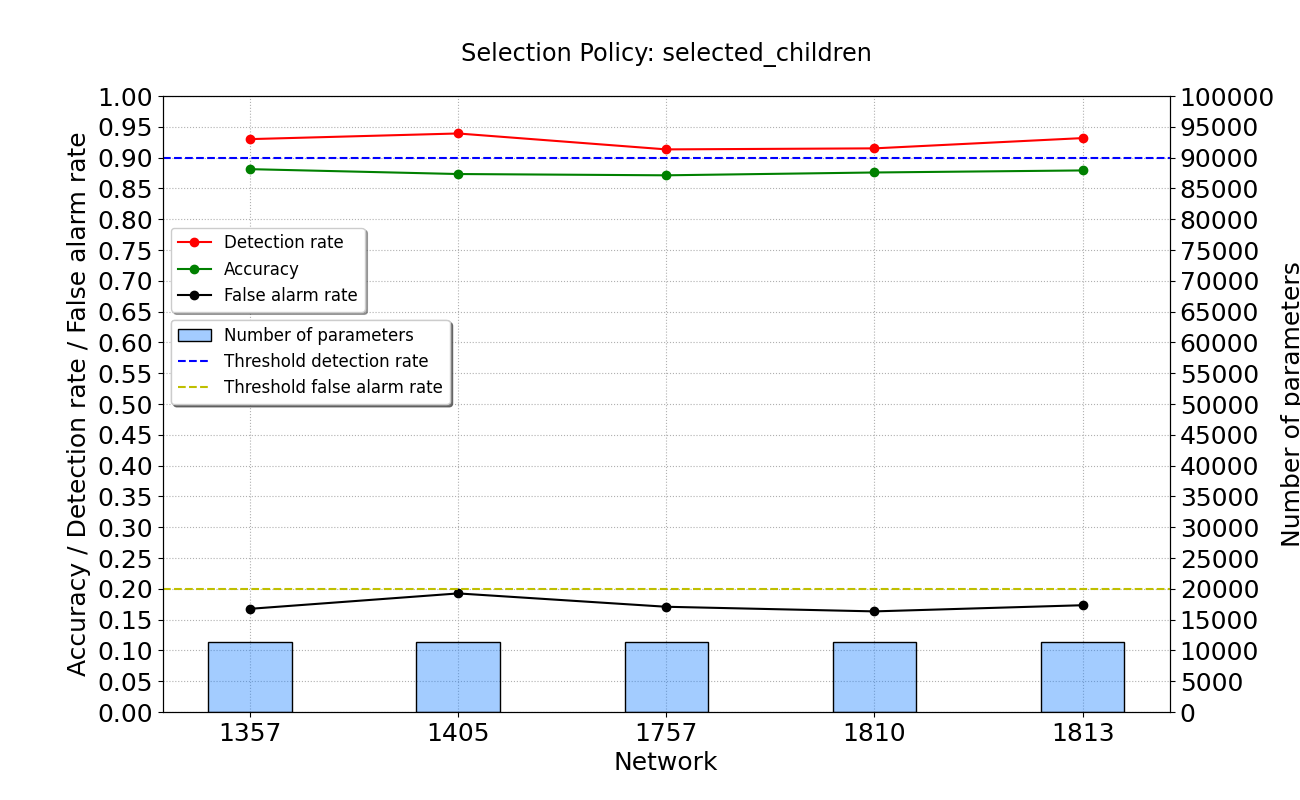
\includegraphics[width=1.0\linewidth, height=9cm]{BachelorMasterThesis/ExperimentsAndResults/Figures/selected_children/selected_children_networks_least_nop.png}
        \caption{Selected children - network with least parameters for detection rate greater than 90\% and false alarm rate less than 20\%}
        \label{fig:selected_children_networks_least_nop}
    % \begin{minipage}{1.0\textwidth}
    % \end{minipage}%
\end{figure}

This is not the case with the selection strategy - selected children and all children. With selected children, the number of parameters decrease to around 10,000 maintaining the detection rate of greater than 90\% and false alarm rate less than 20\% (Figure~\ref{fig:selected_children_networks_least_nop}). With all children, the number of parameters further decrease with many networks having parameters less than 10,000 maintaining the constrains on detection rate and false alarm rate (Figure~\ref{fig:all_children_networks_least_nop}, Figure~\ref{fig:all_children_networks_least_nop_all_less_than_10000}). These networks have less than one fourth of the number of parameters of the seed model.

The selection strategy of lemonade produces the best accuracy for a network at 98.6\% (table \ref{table:network_with_highest_acc}). This network has a very high detection rate and low false alarm rate, but also has higher number of parameters compared to selected children and all children. For the network with minimum number of parameters with detection rate greater than 90\% and false alarm rate less than 20\%, this strategy produces a network with 18,163 parameters. This network has better accuracy, detection rate and false alarm rate than all the other selection policies but it also has higher number of parameters than selected children and all children. 

\begin{figure}[ht!]
    \centering
        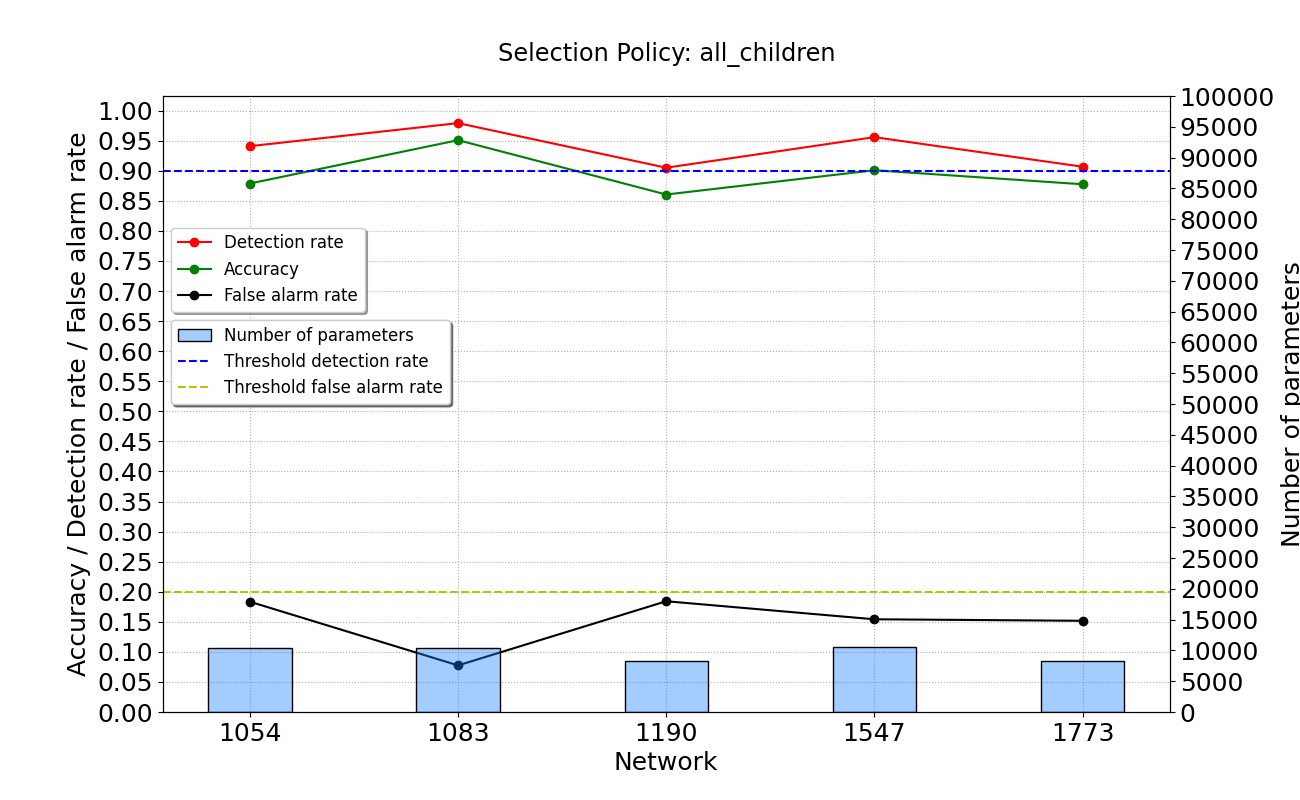
\includegraphics[width=1.0\linewidth, height=9cm]{BachelorMasterThesis/ExperimentsAndResults/Figures/all_children/all_children_networks_least_nop.png}
        \caption{All children - network with least parameters for detection rate greater than 90\% and false alarm rate less than 20\%}
        \label{fig:all_children_networks_least_nop}
    % \begin{minipage}{1.0\textwidth}
    % \end{minipage}%
\end{figure}

\begin{figure}[ht!]
    \centering
        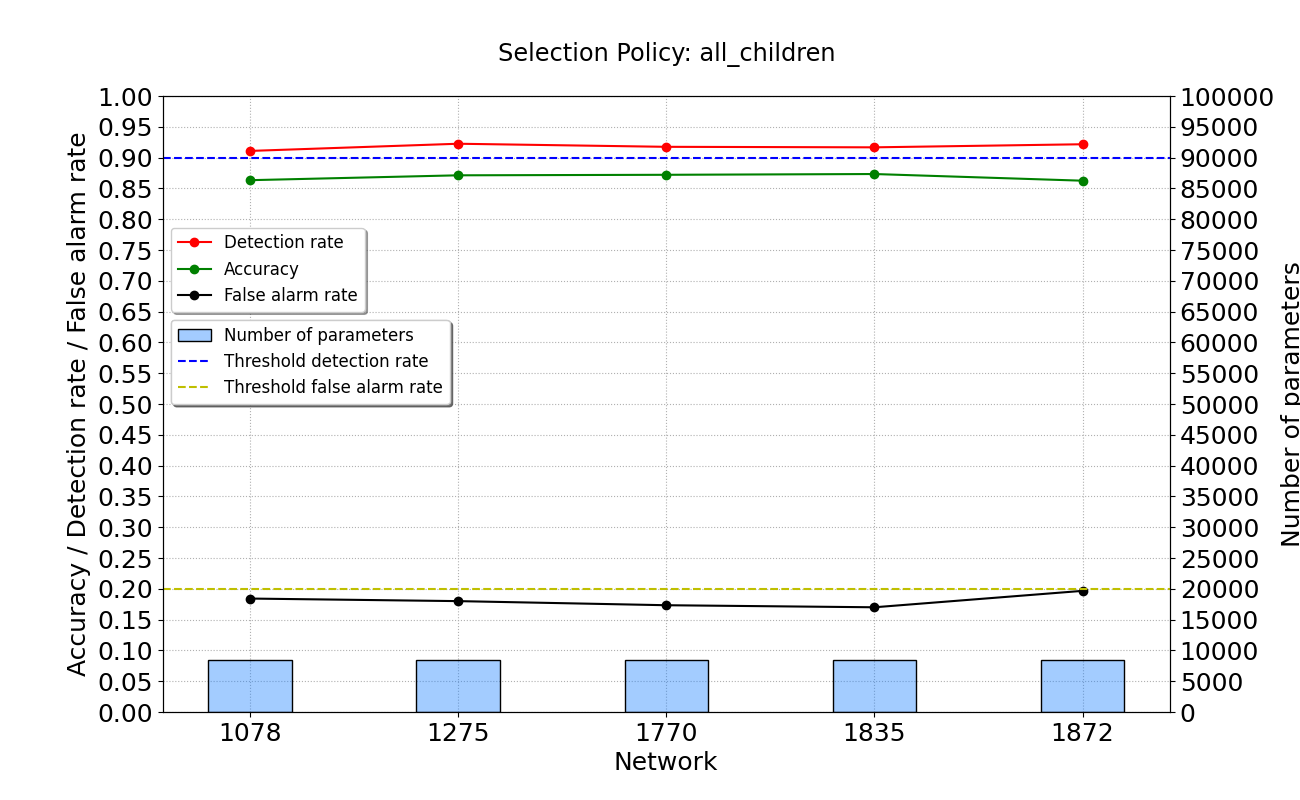
\includegraphics[width=1.0\linewidth, height=8cm]{BachelorMasterThesis/ExperimentsAndResults/Figures/all_children/all_children_networks_least_nop_all_less_than_10000.png}
        \caption{All children - networks with parameters less than 10,000 for detection rate greater than 90\% and false alarm rate less than 20\%}
        \label{fig:all_children_networks_least_nop_all_less_than_10000}
    % \begin{minipage}{1.0\textwidth}
    % \end{minipage}%
\end{figure}

Further results for the selection policies are described in table \ref{table:network_with_highest_acc} and table \ref{table:network_with_min_nop}. Table \ref{table:network_with_highest_acc} shows the network with the highest accuracy for all the selection policies with other respective metrics of that network, where as table \ref{table:network_with_min_nop} displays the network with the least number of parameters for detection rate greater than 90\% and false alarm rate less than 20\%. These are the cumulative results for all the experiments performed. These results indicate that for both accuracy and for number of parameters, we get better results using the NAS process when compared to the seed models.

\begingroup
\setlength{\tabcolsep}{4pt}
\renewcommand{\arraystretch}{1.2}
\begin{table}[ht!]
\normalsize
\resizebox{\textwidth}{!}{%
\begin{tabular}{|c|c|c|c|c|c|}
\hline
\textbf{\begin{tabular}[c]{@{}c@{}}Selection \\ strategy\end{tabular}} &
  \textbf{\begin{tabular}[c]{@{}c@{}}Generation \\ Number\end{tabular}} &
  \textbf{Accuracy} &
  \textbf{\begin{tabular}[c]{@{}c@{}}Number \\ of \\ parameters\end{tabular}} &
  \textbf{\begin{tabular}[c]{@{}c@{}}Detection\\ Rate\end{tabular}} &
  \textbf{\begin{tabular}[c]{@{}c@{}}False\\ Alarm\\ Rate\end{tabular}} \\ \hline
\textbf{Aging}  & 24 & 0.981 & 98,849 & 0.984 & 0.023 \\ \hline
\textbf{\begin{tabular}[c]{@{}c@{}}Selected\\ children\end{tabular}} & 3 & 0.985 & 64,673 & 0.985 & 0.014 \\ \hline
\textbf{\begin{tabular}[c]{@{}c@{}}All\\ children\end{tabular}}      & 2 & 0.989 & 69,113 & 0.985 & 0.007 \\ \hline
\textbf{\begin{tabular}[c]{@{}c@{}}Lemonade\end{tabular}}      & 19 & 0.986 & 72,249 & 0.99 & 0.019 \\ \hline
\end{tabular}}
\caption{Networks for selection strategy with maximum accuracy}
\label{table:network_with_highest_acc}
\end{table}
\endgroup

\begingroup
\setlength{\tabcolsep}{4pt}
\renewcommand{\arraystretch}{1.2}
\begin{table}[ht!]
\normalsize
\resizebox{\textwidth}{!}{%
\begin{tabular}{|c|c|c|c|c|c|}
\hline
\textbf{\begin{tabular}[c]{@{}c@{}}Selection \\ strategy\end{tabular}} &
  \textbf{\begin{tabular}[c]{@{}c@{}}Generation \\ Number\end{tabular}} &
  \textbf{\begin{tabular}[c]{@{}c@{}}Number \\ of \\ parameters\end{tabular}} &
  \textbf{Accuracy} &
  \textbf{\begin{tabular}[c]{@{}c@{}}Detection\\ Rate\end{tabular}} &
  \textbf{\begin{tabular}[c]{@{}c@{}}False\\ Alarm\\ Rate\end{tabular}} \\ \hline
\textbf{Aging}  & 81 & 26,409 & 0.877 & 0.939 & 0.185 \\ \hline
\textbf{\begin{tabular}[c]{@{}c@{}}Selected\\ children\end{tabular}} & 98 & 11,219 & 0.893 & 0.903 & 0.117 \\ \hline
\textbf{\begin{tabular}[c]{@{}c@{}}All\\ children\end{tabular}}      & 59 & 8,273 & 0.860 & 0.905 & 0.184 \\ \hline
\textbf{\begin{tabular}[c]{@{}c@{}}Lemonade\end{tabular}}      & 50 & 18,163 & 0.936 & 0.932 & 0.059 \\ \hline
\end{tabular}}
\caption{Networks with minimum number of parameters for detection rate greater than 90\% and false alarm rate less than 20\%}
\label{table:network_with_min_nop}
\end{table}
\endgroup
